\section{Evaluation}
\label{sec:evaluation}

% In this section, we analyze the performance of our algorithm
% to check the equivalence of context-free session types. 
% To do so, 

%Armed with the results in section~\ref{sec:algorithm}, we decided to
%benchmark the algorithm on a test suite of carefully crafted pair of
%types (more on this in section~\ref{sec:evaluation}). During this 
%process we came across a pair of types,



We implemented the algorithm
% we have presented thus far (sketched in
% Listings~\ref{lst:toGrammar}, \ref{lst:prune}, \ref{lst:algorithm})
in Haskell and used the Glasgow Haskell Compiler, GHC version 8.6.3,
from which we have obtained the running times we present in this
section.  Evaluation was conducted on a Mac mini equipped with a 3.6
GHz Intel Core i3, 8 GB of memory, and running MacOS 10.14.3.
%

Once the proposals for improvement of the algorithm were established,
we have benchmarked the algorithm on a test suite of carefully crafted 
pair of types. These tests comprise valid and invalid equivalences, 
for a total of 138 tests. We have profiled our program for the
time and memory allocated during the tests. For this purpose,
we have used GHC's profiling feature, that maintains a cost-centre stack
to keep track of the incurred costs. We ran the tests 10 times, 
kept a record of the run time and memory allocated for each run,
discarded the best and worst values obtained and, then, we have 
measured the average of the remaining values. The results are 
depicted in figure~\ref{fig:results}.

\begin{figure}[h]
	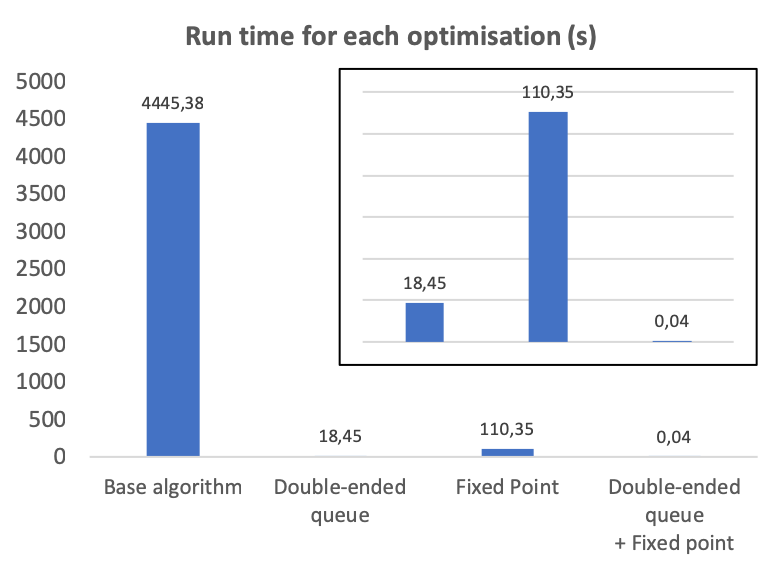
\includegraphics[height=5cm]{img/run_time}	\enspace 
	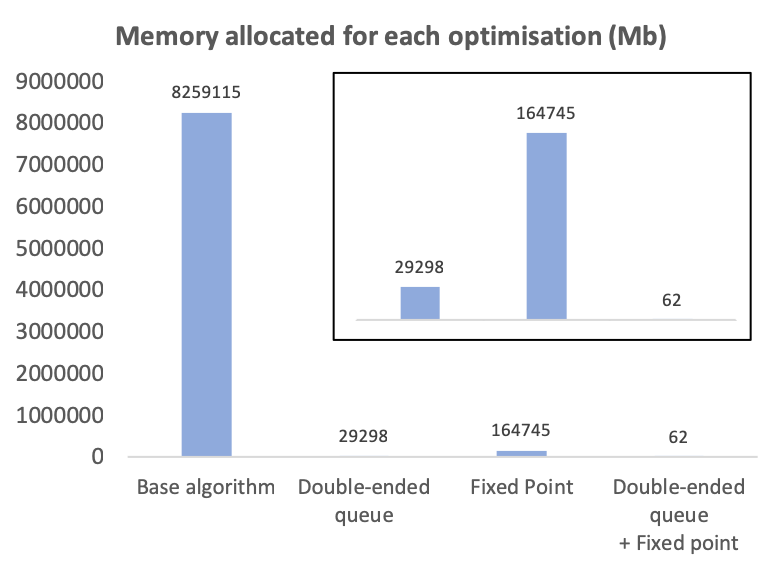
\includegraphics[height=5cm]{img/memory_alloc}	
	\caption{Test results: running times (on the left) and
	memory allocated (on the right) checking the equivalence 
	of context-free session types in 138 tests.}
	\label{fig:results}
\end{figure}

For the base algorithm, proposed in listing~\ref{lst:algorithm},
we have obtained an average running time of about 4445,38 seconds
and 8259115 Mb memory allocated. From the moment we introduced 
optimizations in the algorithm the results have improved remarkably:
iterating the simplification phase in the search for a fixed point 
allowed to reduce the value of the running time to 110,35 seconds and 
the memory allocated to 164745 Mb, whereas the implementation of the 
double-ended queue allowed to reduce the running time to 18,45 seconds 
and the allocated memory to 29298. The combination of both exhibit an 
improvement on more than 12,000,000\% of the base case, by 
achieving an average of 0,04 seconds for the running time and 62 Mb 
of allocated memory.

The running times and memory allocated are presented in
Figure~\ref{fig:results}, exhibit an improvement on more than
12,000,000\%. 

The running time of example in~\eqref{ex:chaotic} was
brought down to 0.008 seconds. For this reasons, our
proposal for an algorithm to check the equivalence of context-free
session types stands on adapting the simplification stage to enable
double-ended enqueueing and the computation of a fixed point at the
simplification phase Listing~\ref{lst:enhanced} presents an enhanced
version of the simplification stage coping the new proposals.



%%% Local Variables:
%%% mode: latex
%%% TeX-master: "main"
%%% End:
